%-------------------------------------------------------------------------------
% Supplementary Material for the three-way TCRE comparison.
% Builds with the same preview/MDPI toggle as main.tex.
%-------------------------------------------------------------------------------

\newif\ifpreview
\previewtrue   % flip with main.tex

\ifpreview
\documentclass[10pt,a4paper]{article}
\usepackage[margin=2.5cm]{geometry}
\usepackage[utf8]{inputenc}
\usepackage[T1]{fontenc}
\usepackage{lmodern}
\usepackage{amsmath,amssymb,amsfonts}
\usepackage{graphicx}
\usepackage{booktabs}
\usepackage{xcolor}
\usepackage{hyperref}
\usepackage{enumitem}
\usepackage{caption}
\usepackage{float}
\usepackage{multirow}
\usepackage{textgreek}
\providecommand{\upmu}{\textmu}
\hypersetup{colorlinks=true, linkcolor=black, citecolor=blue, urlcolor=blue}
\setlist[itemize]{leftmargin=1.4em, itemsep=2pt, topsep=4pt}
\else
\documentclass[sensors,article,submit,pdftex,moreauthors]{Definitions/mdpi}
\firstpage{S1}
\fi

\newcommand{\TBD}[1]{{\color{red}\textbf{[TBD: #1]}}}
\newcommand{\NOTE}[1]{{\color{blue}\textit{[note: #1]}}}

\title{Supplementary Material:\\
A Methods-Harmonized Comparison of Tripolar Concentric Ring Electrode Constructions for Non-Invasive EEG}
\author{Shayan Khodabakhsh and co-authors}
\date{}

\begin{document}
\maketitle

%-------------------------------------------------------------------------------
\section{S1.\quad Sensitivity Analysis Across Pipeline Variants}\label{sec:s1}

The main text reports results under preprocessing variant B (60~Hz notch + zero-phase FIR 0.05--55~Hz bandpass). To check that our conclusions are not pipeline-specific, we re-ran the cohort under two additional variants:

\begin{itemize}
\item \textbf{Variant A}: notch + bandpass + Daubechies-8 level-3 wavelet denoising + per-epoch z-score (the original gel-TCRE pipeline).
\item \textbf{Variant B}: notch + bandpass only (\textbf{primary}, used in main text).
\item \textbf{Variant C}: notch only (no bandpass).
\end{itemize}

Figure~S1 shows the cohort-level sensitivity of the three main-text endpoints (alpha SNR, alpha reactivity, spectrogram SSIM) under each variant. Per-class medians under variants A, B, and C are identical to the precision reported (Table~S1). Two reasons: (i)~all three primary endpoints are ratios (SNR is a between-band log-ratio; reactivity is a between-condition power ratio; SSIM is a normalised image-similarity index) and are therefore invariant under the linear z-score that distinguishes variant~A from variant~B; (ii)~the 0.05--55~Hz bandpass that distinguishes variants A and B from variant~C neither removes nor reshapes the 8--13~Hz band that drives the alpha endpoints. The conclusions reported in §3 of the main text consequently hold across all three variants. A complementary single-subject preprocessing-sensitivity check on the excluded gel session is shown in Figure~S2; the tEEG ADC saturation persists across all three variants, supporting the interpretation that the issue is acquisition-side rather than processing-side.

\begin{figure}[H]
\centering
\IfFileExists{figs/sensitivity_abc.png}{%
  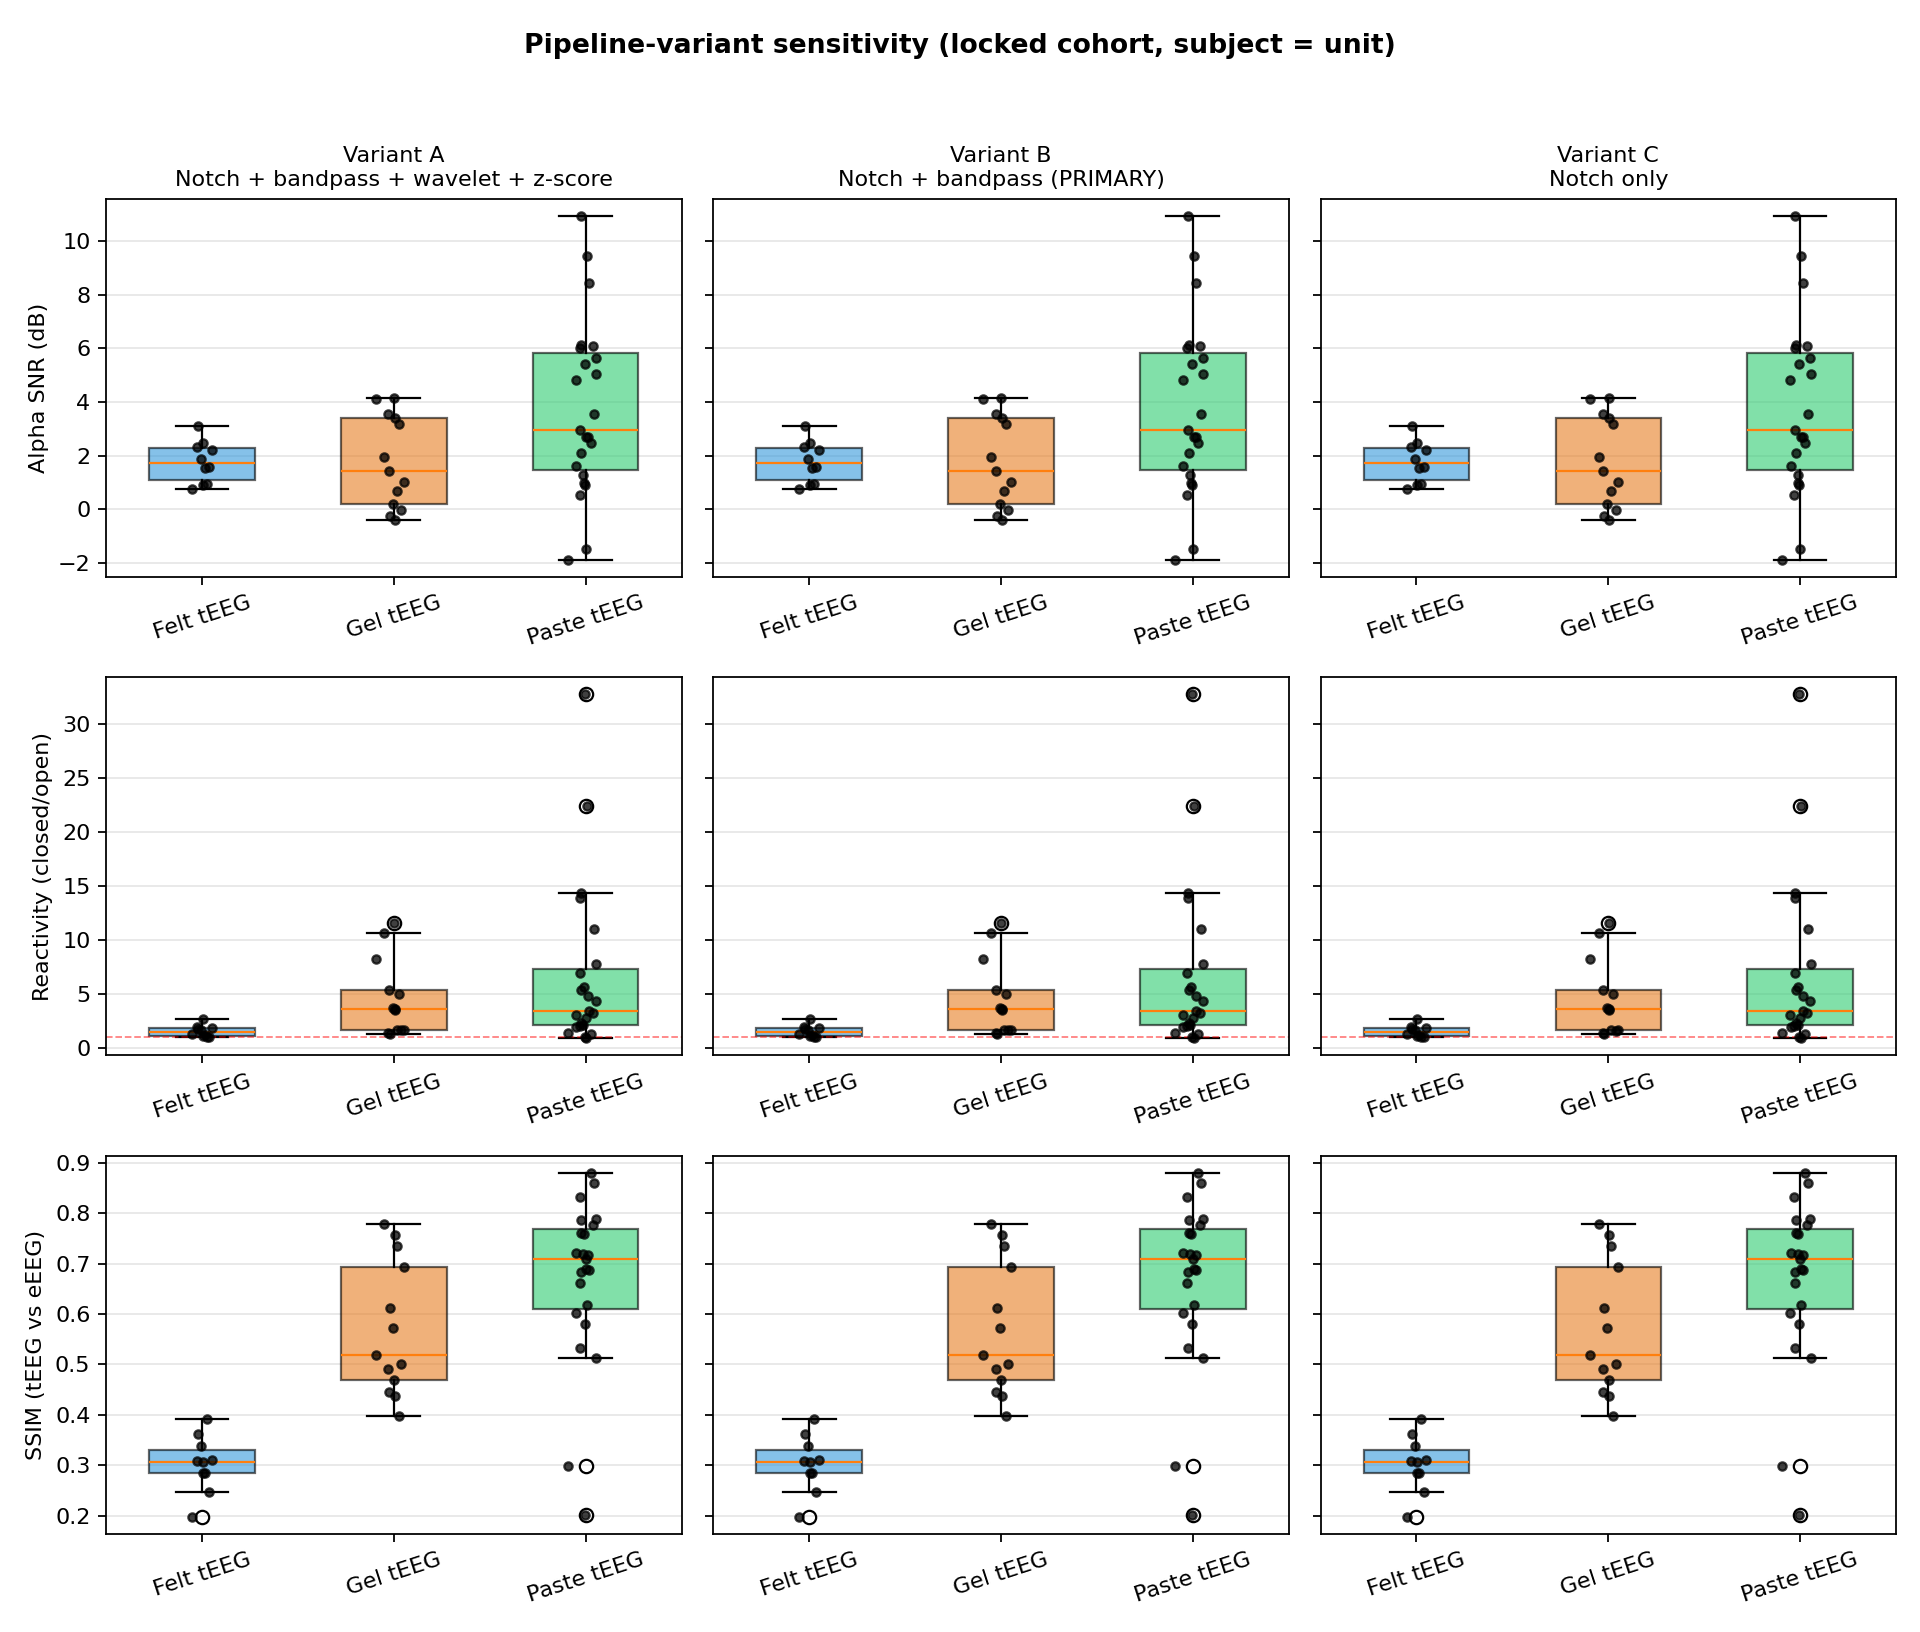
\includegraphics[width=0.98\linewidth]{figs/sensitivity_abc.png}%
}{\fbox{\parbox{0.7\linewidth}{\centering\vspace{1em}\textit{figure missing --- run \texttt{python paper\_sensors/build\_sensitivity\_figure.py}}\vspace{1em}}}}
\caption*{\textbf{Figure S1.} Cohort-level pipeline-variant sensitivity. Rows: alpha SNR, alpha reactivity, spectrogram SSIM. Columns: variants A (notch + bandpass + wavelet + z-score), B (notch + bandpass; primary), C (notch only). Subject is the unit of analysis. The three primary endpoints are robust to pipeline variant by design (see §S1 prose). Auto-generated by \texttt{build\_sensitivity\_figure.py}.}
\end{figure}

\begin{table}[H]
\caption*{\textbf{Table S1.} Per-class median under each variant, $n$ subjects in parentheses. Auto-generated by \texttt{build\_sensitivity\_figure.py}; see \texttt{paper\_sensors/sensitivity\_abc.md} for the full breakdown across all three endpoints.}
\centering\small
\begin{tabular}{lccc}
\toprule
\textbf{Class} & \textbf{Variant A} & \textbf{Variant B} & \textbf{Variant C} \\
\midrule
\multicolumn{4}{l}{\emph{Alpha SNR (dB)}}\\
Felt tEEG  & 1.72 ($n=10$) & 1.72 ($n=10$) & 1.72 ($n=10$) \\
Gel tEEG   & 1.43 ($n=13$) & 1.43 ($n=13$) & 1.43 ($n=13$) \\
Paste tEEG & 2.97 ($n=23$) & 2.97 ($n=23$) & 2.97 ($n=23$) \\
\midrule
\multicolumn{4}{l}{\emph{Reactivity (closed/open)}}\\
Felt tEEG  & 1.49 ($n=10$) & 1.49 ($n=10$) & 1.49 ($n=10$) \\
Gel tEEG   & 3.63 ($n=13$) & 3.63 ($n=13$) & 3.63 ($n=13$) \\
Paste tEEG & 3.43 ($n=23$) & 3.43 ($n=23$) & 3.43 ($n=23$) \\
\midrule
\multicolumn{4}{l}{\emph{SSIM (tEEG vs eEEG)}}\\
Felt  & 0.31 ($n=10$) & 0.31 ($n=10$) & 0.31 ($n=10$) \\
Gel   & 0.52 ($n=13$) & 0.52 ($n=13$) & 0.52 ($n=13$) \\
Paste & 0.71 ($n=23$) & 0.71 ($n=23$) & 0.71 ($n=23$) \\
\bottomrule
\end{tabular}
\end{table}

\begin{figure}[H]
\centering
\IfFileExists{figs/gel_vep_excluded_sensitivity.png}{%
  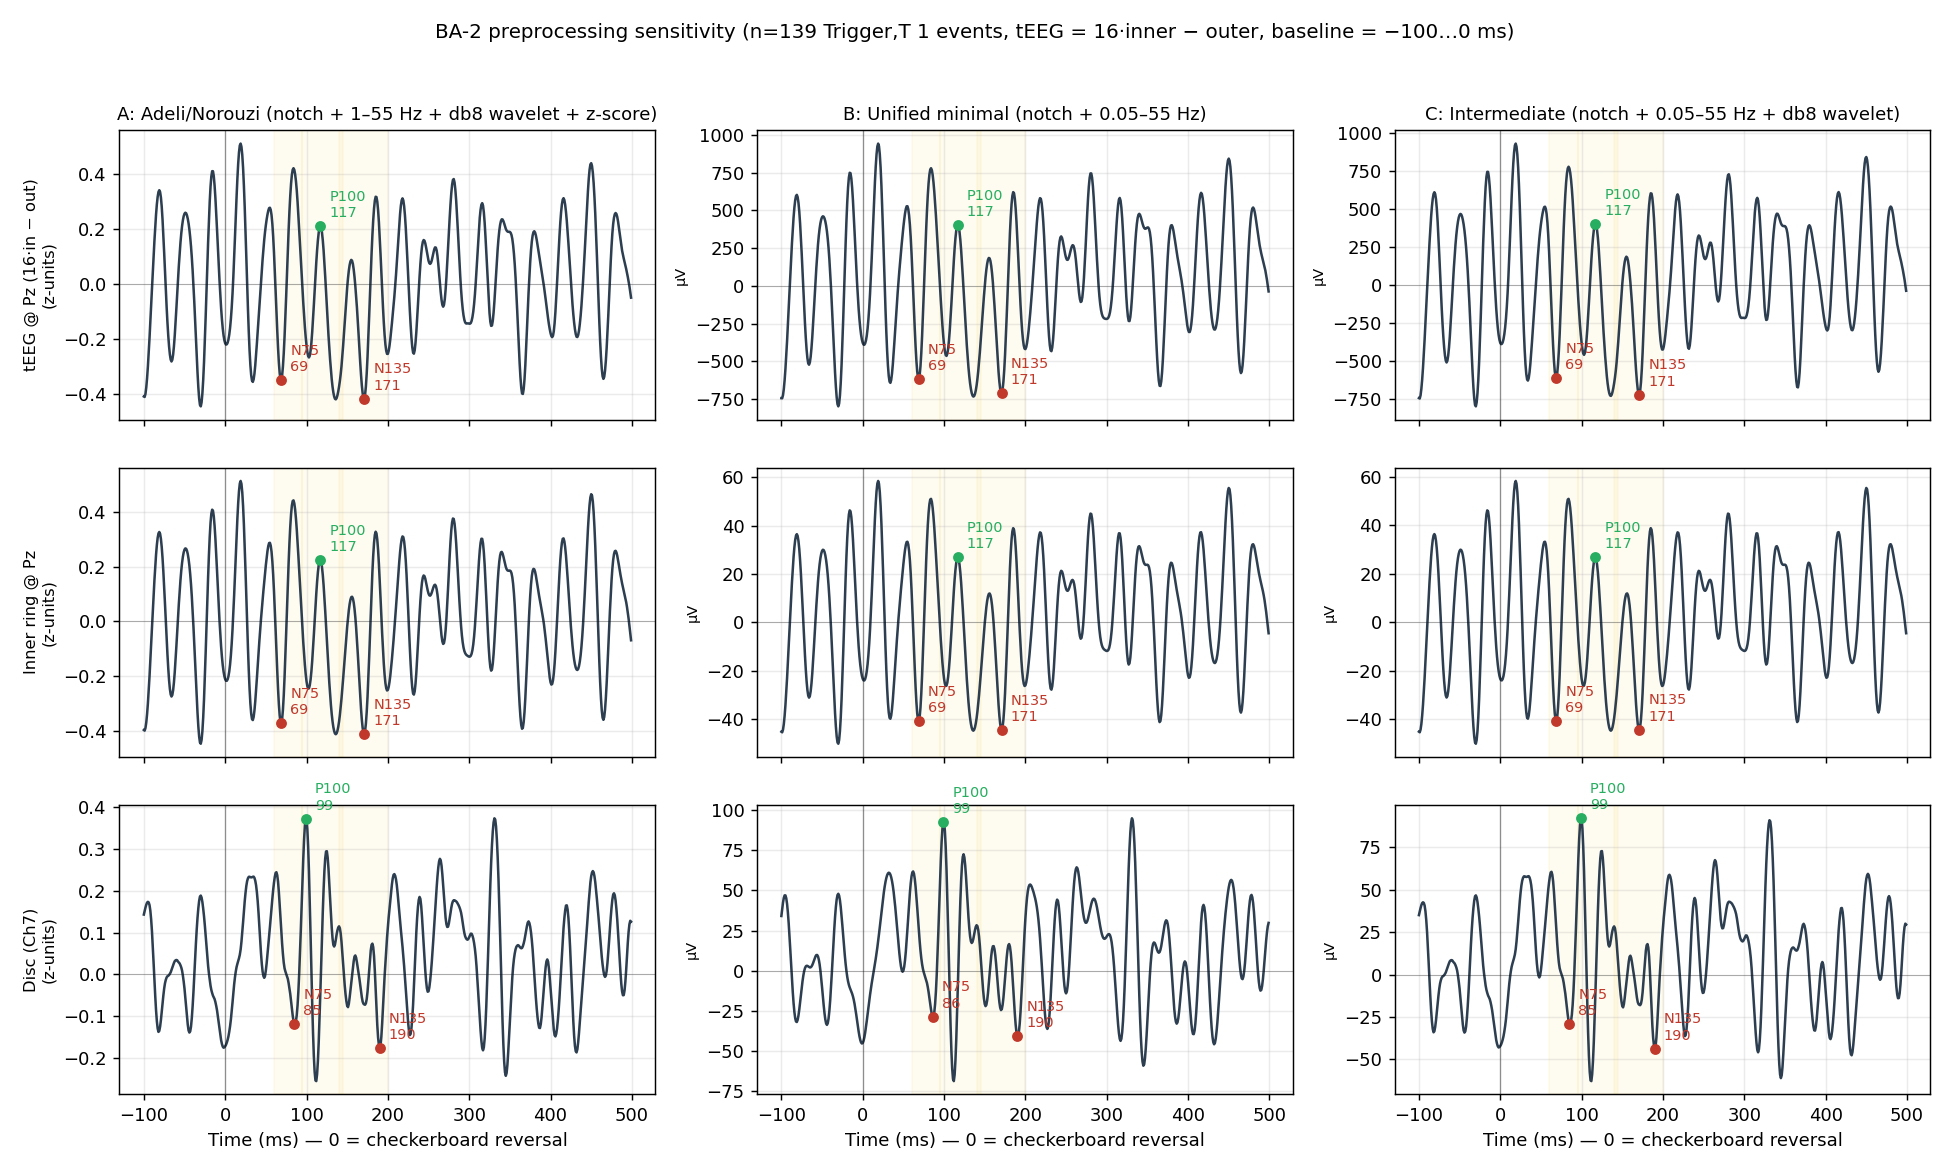
\includegraphics[width=0.95\linewidth]{figs/gel_vep_excluded_sensitivity.png}%
}{\fbox{\parbox{0.7\linewidth}{\centering\vspace{1em}\textit{figure missing}\vspace{1em}}}}
\caption*{\textbf{Figure S2.} Excluded gel session VEP under pipeline variants A / B / C. ADC saturation persists across variants, indicating an acquisition-side rather than processing-side cause.}
\end{figure}

%-------------------------------------------------------------------------------
\section{S2.\quad Full Per-Subject QC Tables}\label{sec:s2}

Table~S3 expands the main-text QC summary into the full per-channel breakdown for every subject in the analysis cohort, with channel-level clipping percentages and the per-channel inclusion decision made by the QC pipeline. The auto-generated CSV behind this table is at \texttt{paper/qc\_full.csv}.

%-------------------------------------------------------------------------------
\section{S3.\quad Gel-Cohort VEP Sanity Check (Qualitative)}\label{sec:s3}

Three gel-cohort recordings were re-processed through the harmonized pipeline to characterise the gel-VEP behaviour underlying the cross-construction VEP exclusion in main-text §3.7: G02 and G10 (both in the analysis cohort) plus one additional gel session that failed cohort QC due to continuous tEEG ADC-rail saturation (the ``excluded session''). G02 produces a marginally recognisable VEP morphology on tEEG. The excluded session's tEEG hits the INT16 ADC rail while its paired Pz disc still produces a recognisable evoked response. G10 is the cleanest of the three, with N75/P100/N135 visible on tEEG at Pz and matching morphology on the paired Pz disc at smaller amplitude. The unified-pipeline overview across the three sessions shows the heterogeneity in VEP recoverability that motivates excluding the gel cohort from cross-construction VEP statistics.

\begin{figure}[H]
\centering
\IfFileExists{figs/gel_vep_G02.png}{%
  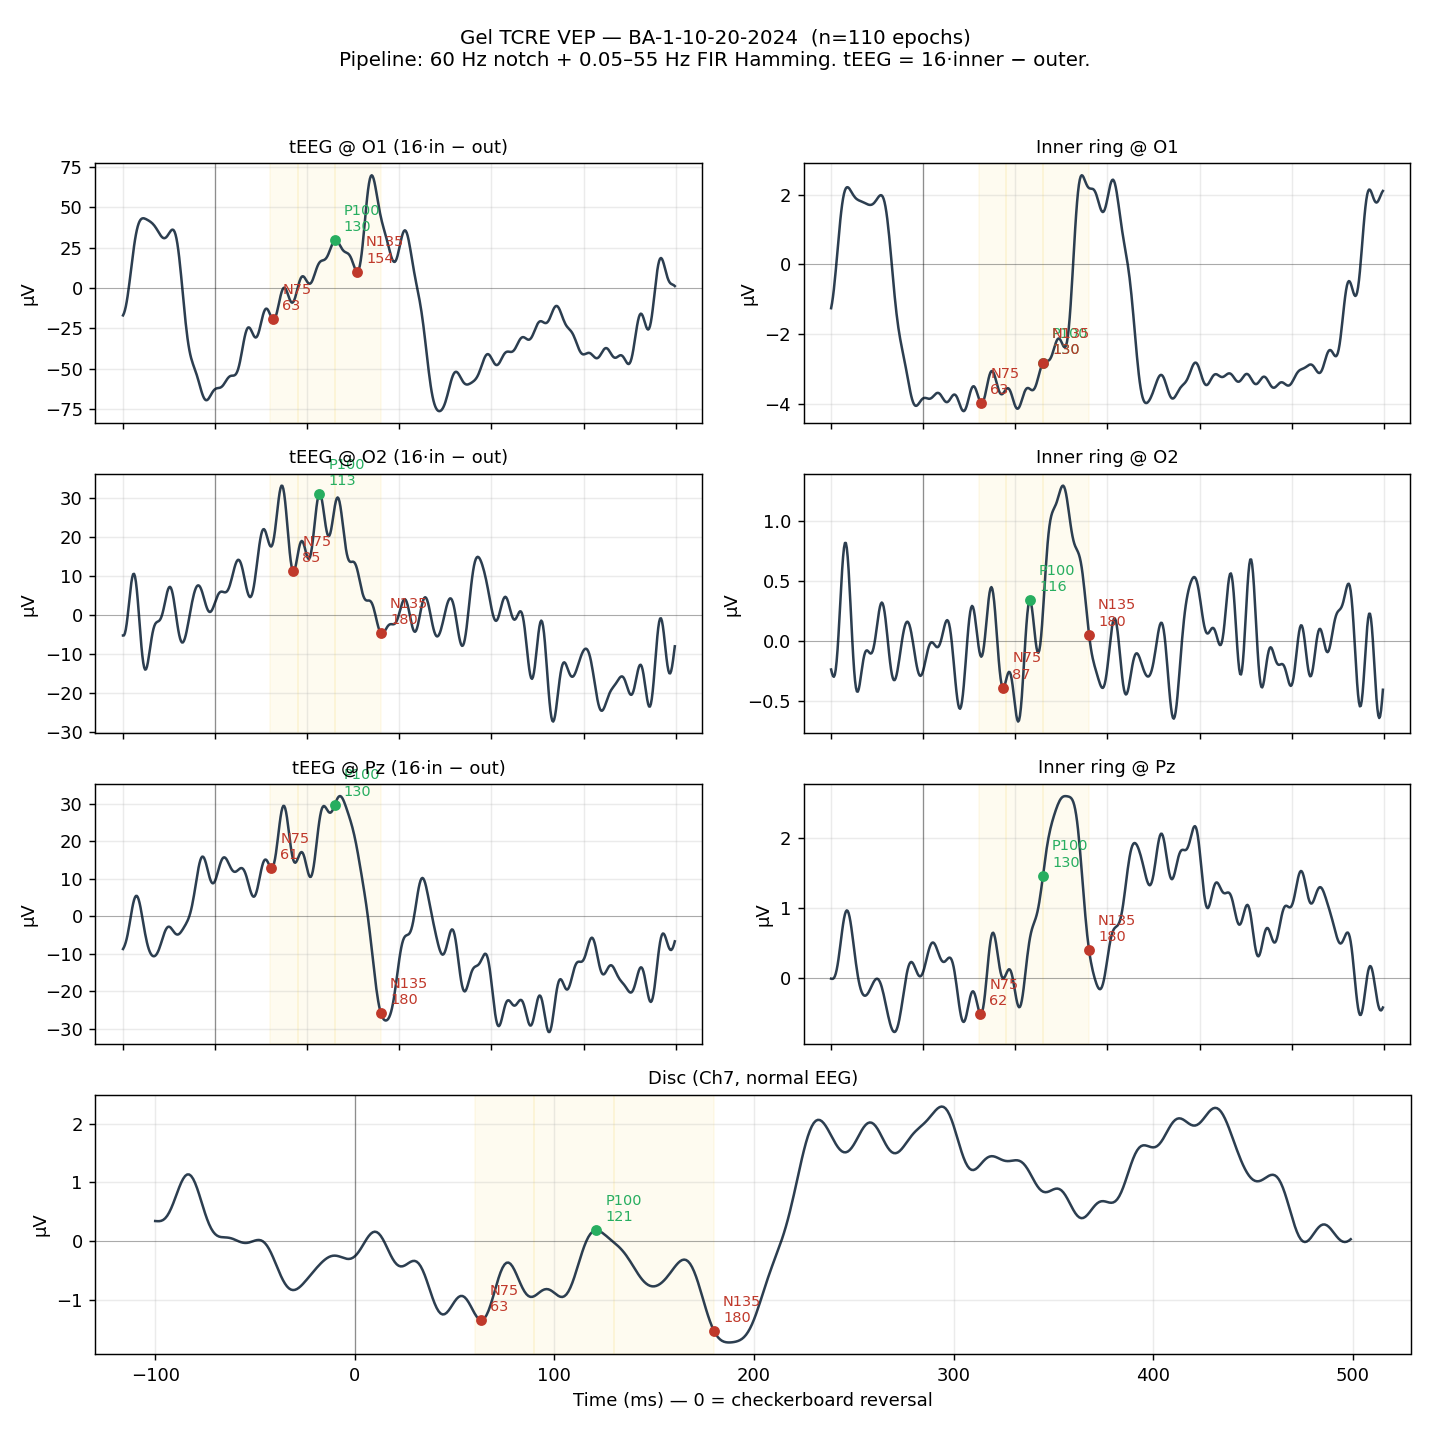
\includegraphics[width=0.92\linewidth]{figs/gel_vep_G02.png}%
}{\fbox{\parbox{0.6\linewidth}{\centering\vspace{1em}\textit{figure missing}\vspace{1em}}}}
\caption*{\textbf{Figure S3.} Subject G02, harmonized pipeline.}
\end{figure}

\begin{figure}[H]
\centering
\IfFileExists{figs/gel_vep_excluded.png}{%
  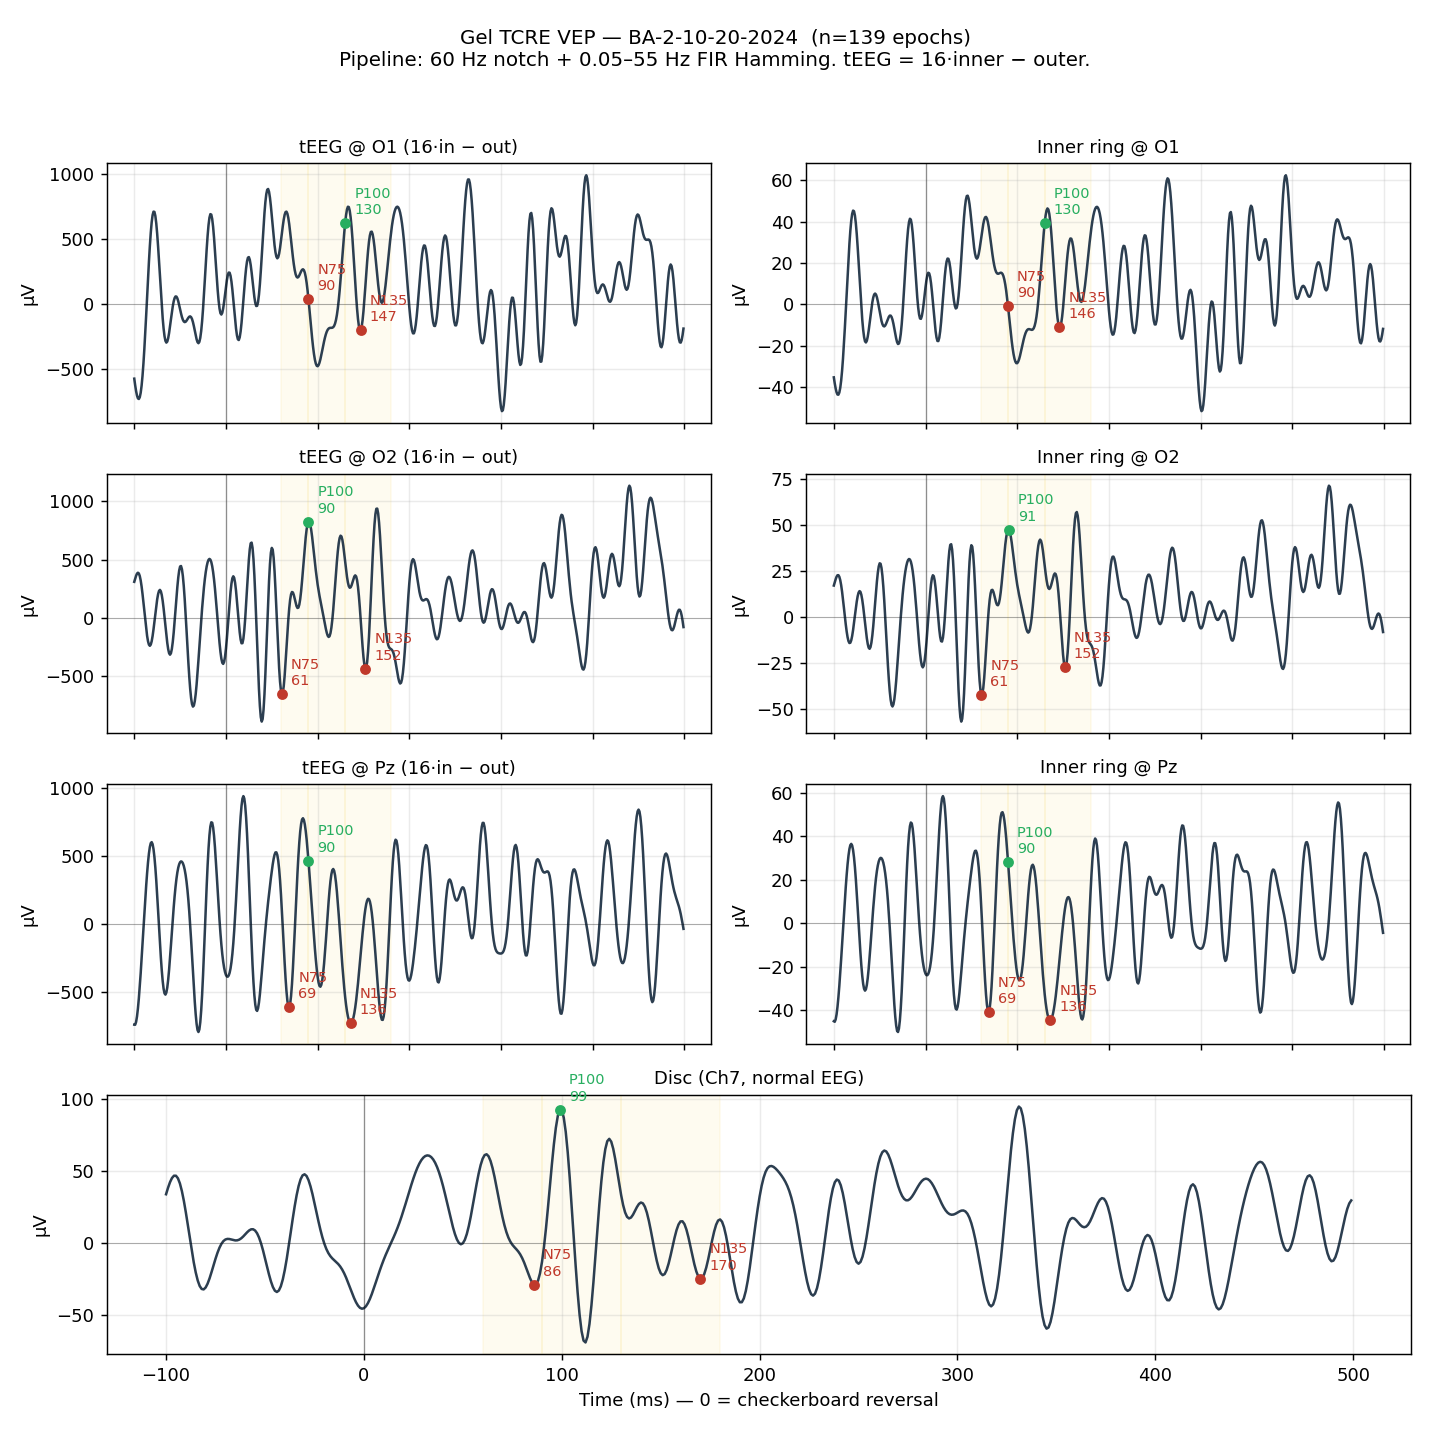
\includegraphics[width=0.92\linewidth]{figs/gel_vep_excluded.png}%
}{\fbox{\parbox{0.6\linewidth}{\centering\vspace{1em}\textit{figure missing}\vspace{1em}}}}
\caption*{\textbf{Figure S4.} Excluded gel session. tEEG hits the INT16 ADC rail; paired Pz disc still produces a recognisable VEP.}
\end{figure}

\begin{figure}[H]
\centering
\IfFileExists{figs/gel_vep_G10.png}{%
  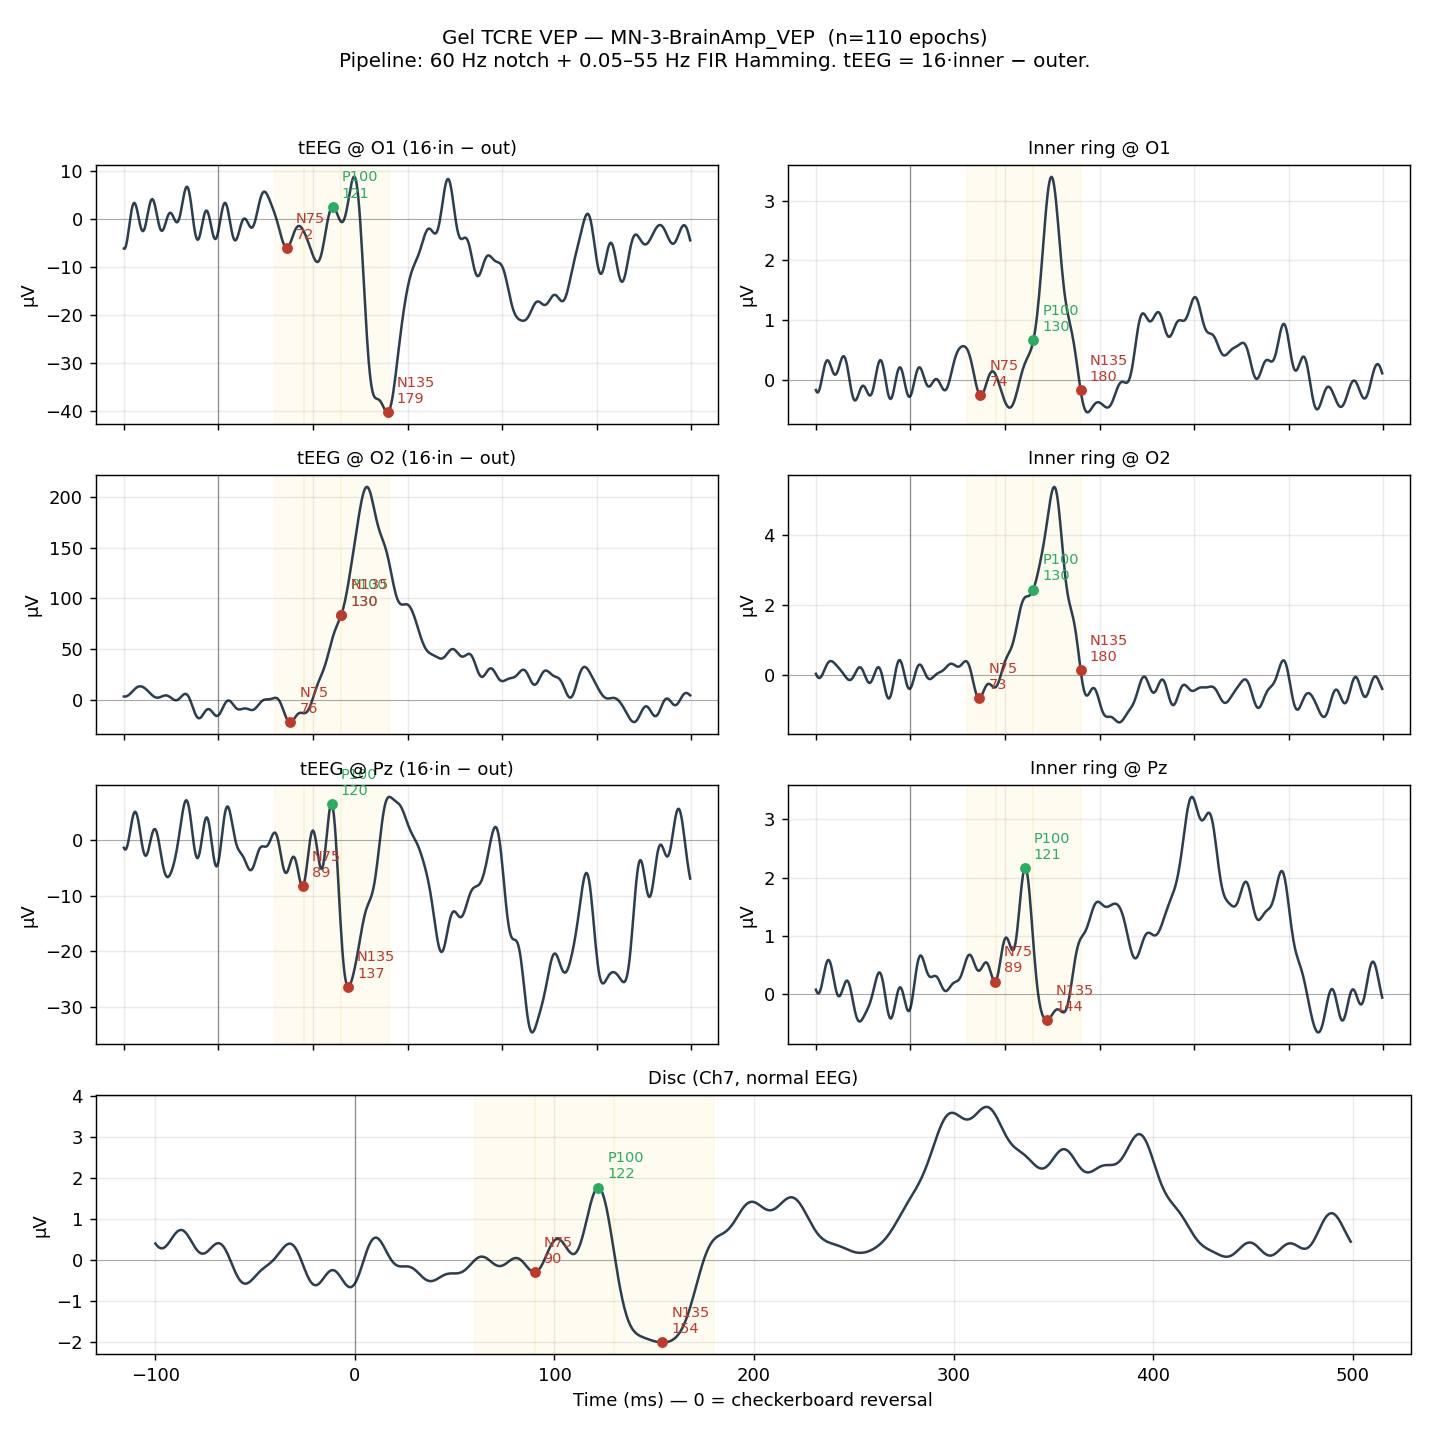
\includegraphics[width=0.92\linewidth]{figs/gel_vep_G10.png}%
}{\fbox{\parbox{0.6\linewidth}{\centering\vspace{1em}\textit{figure missing}\vspace{1em}}}}
\caption*{\textbf{Figure S5.} Subject G10. N75/P100/N135 visible on tEEG at Pz with matching morphology on the paired Pz disc.}
\end{figure}

\begin{figure}[H]
\centering
\IfFileExists{figs/gel_vep_unified.png}{%
  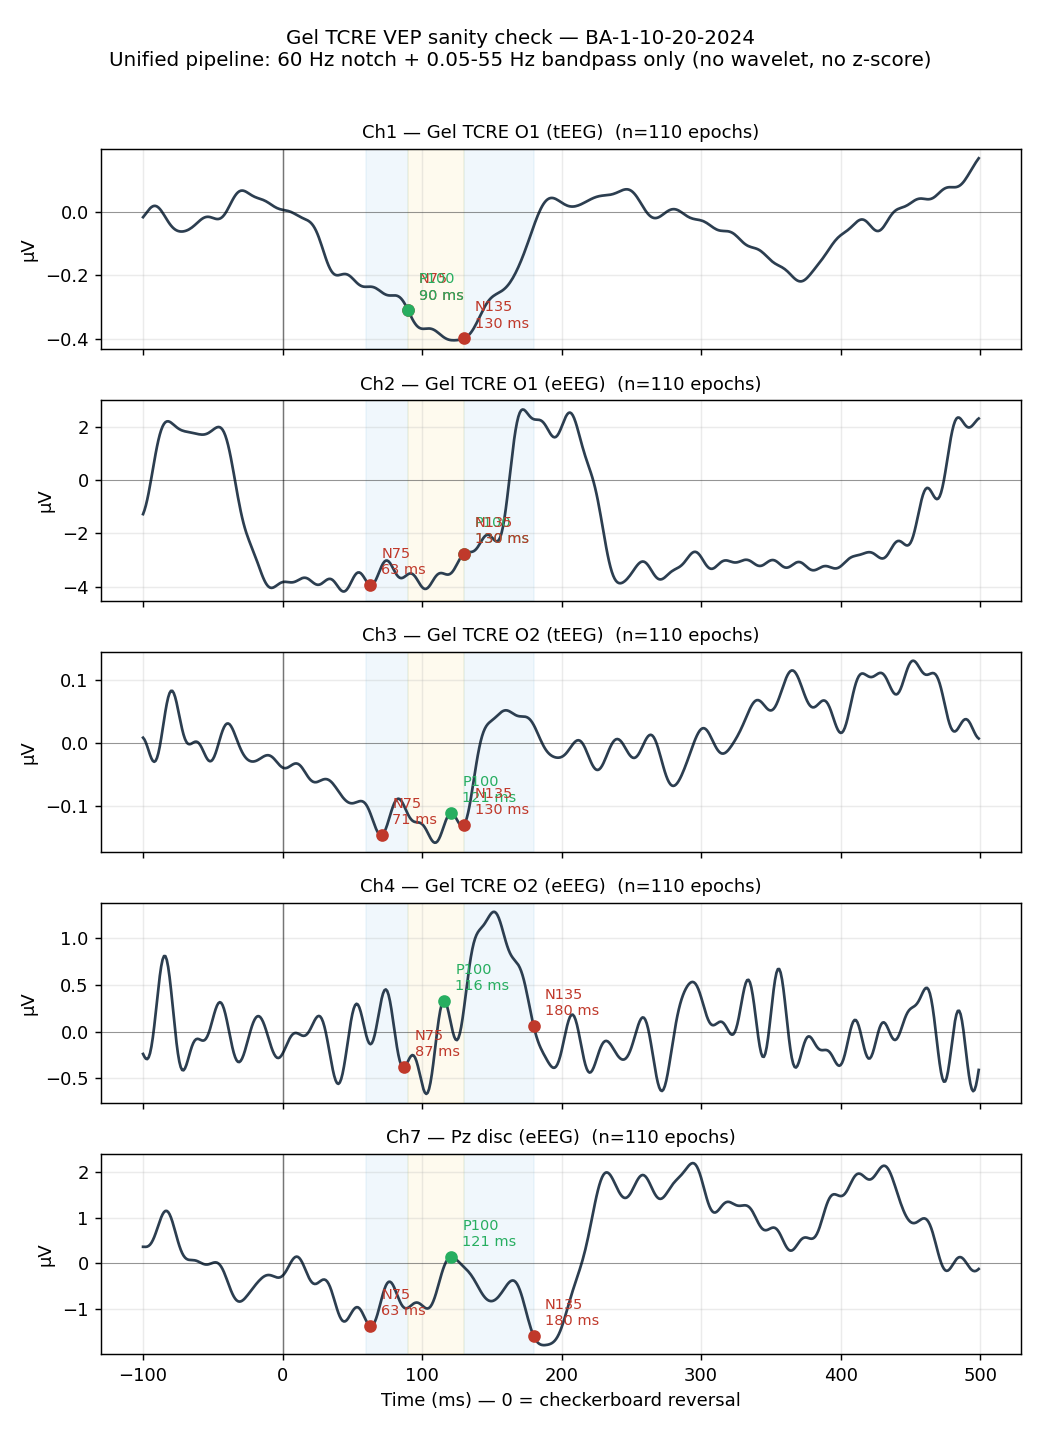
\includegraphics[width=0.92\linewidth]{figs/gel_vep_unified.png}%
}{\fbox{\parbox{0.6\linewidth}{\centering\vspace{1em}\textit{figure missing}\vspace{1em}}}}
\caption*{\textbf{Figure S6.} Unified-pipeline overview across the three gel-VEP sanity-check sessions.}
\end{figure}

%-------------------------------------------------------------------------------
\section{S4.\quad Channel Maps and Channel Class Mapping}\label{sec:s4}

\textbf{Felt setup (11 channels):} Ch1/2 = Felt TCRE \#1 (tEEG/eEEG); Ch3/4 = Felt TCRE \#2; Ch5/6 = Felt TCRE \#3; Ch7/8 = Felt TCRE \#4; Ch9/10 = Paste TCRE \#5; Ch11 = Paste disc.

\textbf{Gel setup (7 channels):} Ch1/2 = Gel TCRE @ O1 (tEEG/eEEG); Ch3/4 = Gel TCRE @ O2; Ch5/6 = Paste TCRE @ Pz; Ch7 = Paste disc @ Pz.

\textbf{Aggregation by abstract type} (used in main text §3.2--§3.6): FELT\_TEEG, FELT\_EEEG, GEL\_TEEG, GEL\_EEEG, PASTE\_TEEG, PASTE\_EEEG, DISC. The Paste TCRE class spans both setups and is used as the cross-setup bridge.

%-------------------------------------------------------------------------------
\section{S6.\quad Long-Felt vs.\ Short-Felt Sub-Cohort Breakdown}\label{sec:s6}

The main-text felt cohort pools $n=10$ subjects across long-felt ($n=3$: LF01--LF03) and short-felt ($n=7$: SF01--SF07) sessions. Table~S2 reports the three primary endpoints separately for each sub-cohort. The construction-level orderings observed in §3 of the main text (Felt $<$ Gel $<$ Paste for tEEG--eEEG SSIM; comparable Felt and Gel alpha SNR; lower Felt reactivity than Gel and Paste) hold within each sub-cohort, so the pooled analysis is not driven by either sub-cohort alone. The long-felt sub-cohort medians for the felt-tEEG class are slightly higher than the short-felt medians on alpha SNR ($2.19$~dB vs.\ $1.57$~dB) and reactivity ($1.87$ vs.\ $1.31$), consistent with the longer recording duration giving more stable per-subject estimates rather than indicating a construction-level difference. Auto-generated by \texttt{scripts/build\_paper\_stats.py}; see \texttt{paper/auto\_stats.md} for the full machine-readable table.

\begin{table}[H]
\caption*{\textbf{Table S2.} Per-class median (BCa 95\% CI) split by long-felt vs.\ short-felt sub-cohort. Gel and pooled-paste rows are unchanged across the split and are reproduced from main-text §3 for direct comparison.}
\centering\small
\begin{tabular}{llccc}
\toprule
\textbf{Sub-cohort} & \textbf{Class} & \textbf{Alpha SNR (dB)} & \textbf{Reactivity} & \textbf{SSIM} \\
\midrule
\multirow{3}{*}{Long felt ($n=3$)}
  & Felt tEEG  & $2.19$ $[1.54,\,2.31]$ & $1.87$ $[1.22,\,1.91]$ & $0.309$ $[0.285,\,0.310]$ \\
  & Paste tEEG & $5.65$ $[2.71,\,6.03]$ & $4.77$ $[4.31,\,6.88]$ & $0.717$ $[0.662,\,0.789]$ \\
  & Disc       & $6.57$ $[2.96,\,7.04]$ & $5.49$ $[4.72,\,8.03]$ & ---                       \\
\midrule
\multirow{3}{*}{Short felt ($n=7$)}
  & Felt tEEG  & $1.57$ $[0.91,\,2.48]$ & $1.31$ $[1.03,\,1.78]$ & $0.306$ $[0.246,\,0.363]$ \\
  & Paste tEEG & $2.07$ $[1.59,\,4.40]$ & $2.78$ $[2.04,\,3.47]$ & $0.701$ $[0.589,\,0.751]$ \\
  & Disc       & $3.65$ $[2.51,\,5.00]$ & $3.06$ $[2.20,\,5.18]$ & ---                       \\
\bottomrule
\end{tabular}
\end{table}

%-------------------------------------------------------------------------------
\section{S5.\quad Code and Reproducibility}\label{sec:s5}

\begin{itemize}
\item Core engine: \texttt{src/eeg\_analysis.py}; comparison framework: \texttt{src/comparison\_analysis.py}.
\item Statistics for main text §3.2--§3.6 are auto-generated by \texttt{paper\_sensors/build\_paper\_stats.py}; the felt-setup VEP figure and table by \texttt{paper\_sensors/build\_felt\_vep\_figure.py}.
\item Random seed for bootstrap BCa is fixed at 0 in both scripts; rerunning the scripts with the same data reproduces the reported numbers exactly.
\item \TBD{Repository URL once made public-readable.}
\end{itemize}

\end{document}
